\section{Forecasting with machine learning}\label{sec:machine-learning}

Once the webapp and database were operational I moved on to developing machine
learning models that would attempt to forecast the microclimate datapoints for
the following 48 hours based on the general weather forecast data for the
region.
\subsection{LightGBM}

LightGBM is a popular machine learning algorithm developed by Microsoft. I chose
LightGBM as it offers a good balance between performance and training efficiency
compared to similar models such as XGBoost \cite{saha2025}.

Both LightGBM and XGBoost are known as 'Gradient Boosted Machines'. This is a
technique in machine learning that effectively combines many weaker machine
learning models (called weak learners) to create a single highly accurate model.
These models are excellent for tabular data (such as my node and forecast data)
and regularly beat out competing learning algorithms \cite{tuychiev2023}.
LightGBM is also compatible with the m2cgen library that allows the final model
to be converted to JavaScript format, allowing it to work within my webapp. All
these factors made LightGBM a good algorithm for my use case.

To train the machine learning models I installed Python with the LightGBM and
m2cgen libraries as described above on my personal laptop. I then also installed
pandas for data handling purposes.

\subsection{Machine learning process}

I aimed to create ten separate machine learning models, one for each node (node
1 and node 2) and sensor reading (temperature, humidity, wind speed, gust speed
and soil moisture).

Training machine learning models requires inputs (referred to as “features”) and
outputs (referred to as “targets”).  For my models, the features came from the
OpenWeather past \textbf{actual} weather data and the targets came from the node
sensor readings. While training, the ML model can "see" both features and
targets. Figure \ref{fig:machine_diagram} below illustrates steps in the
training process.

\begin{figure}[H]
    \centering
    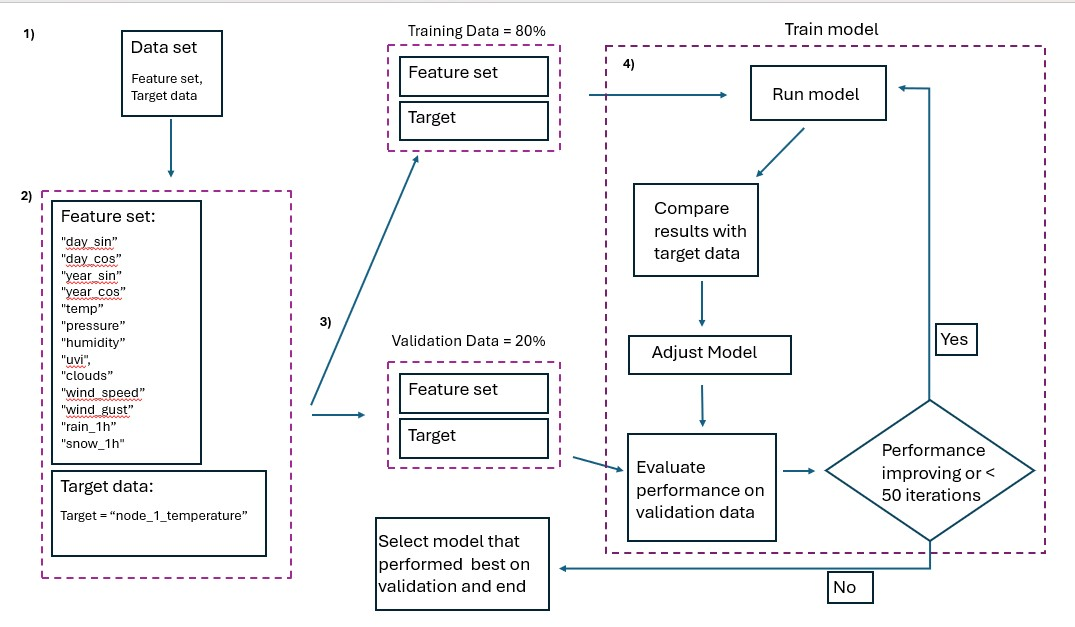
\includegraphics[width=1\textwidth]{contents/part-3/fig3/machine-learning-diagram2.jpg}
    \caption{Infographic showing steps for training with LightGBM. This uses the temperature target for illustration, for other sensor readings the target was changed to that reading}
    \label{fig:machine_diagram}
\end{figure}

The following steps were followed to train each of the ten models.

\begin{enumerate}
    \item Prepare the dataset: A single cleaned dataset was created by matching
          timestamps between the api weather data and the sensor node data. As
          API readings are taken every 10 minutes and node readings every 1
          minute, this meant that 9/10 node readings were discarded. The final
          dataset was roughly 1,400 rows. The data used for training spanned the
          period 15 - 27 August as that final date was when I trained the model.
    \item Define the feature set and target data: The feature set from the
          weather API and targets from the node data were defined, and
          unnecessary columns discarded. The database timestamp field was
          transformed into sine and cosine representations of day and year. This
          is necessary when training on a time-series data set as the algorithm
          must be able to understand the cyclical nature of time. For example,
          using raw timestamps would incorrectly suggest to the algorithm that
          the times of 23:00 on day 1 and 00:00 on day 2 are 23 hours apart
          rather than just 1 hour.
    \item Split the dataset into training data (80\%) and validation data
          (20\%): The data is split by time so the training data consists of the
          first 80\% of the rows and the validation data the last 20\%.  This
          data is then supplied to the model.
    \item Run the iterative training model: For each iteration, the model looks
          at the inputs (training features) and the correct answers (training
          target) of the training rows, and determines where it is getting
          incorrect outputs. It builds a small decision tree that specifically
          aims to correct those mistakes on the training rows and adds that tree
          into itself so its predictions change a little. It then applies the
          updated model to the validation inputs (validation features) and
          compares those predictions to the validation answers (validation
          target) —to see how well the model would do on new "unseen" data. The
          validation data are never used to build the tree; they are only used
          to check the accuracy of the model. If the validation check shows no
          improvement after a number of iterations, the training stops and the
          model keeps the version that performed best on validation.  The
          process will perform a minimum of 50 iterations. I set the maximum
          number of iterations to 250 to prevent the models getting too large,
          as each iteration increases the model size substantially (The humidity
          model is over 40,000 lines long in JavaScript format for example).
\end{enumerate}

Once trained, the final models were uploaded to the backend and the inputs then
came from the OpenWeather \textbf{forecasted} weather data for the next 48 hours
as explained in the following section.


\subsection{Machine learning deployment}

Once the ten models had been trained, they were uploaded to the web server.  I
wrote an automated function on my backend that provides the models with
datapoints from the OpenWeather \textbf{forecast} data for the next 48 hours,
and updates this data every ten minutes to adjust the predictions as the
forecast changes. The outputs from the models are recorded as hourly predictions
for each datapoint in a JSON file, which is requested by the frontend software
and used to display a line graph of predicted values for the next 48 hours.

\begin{figure}[H]
    \centering
    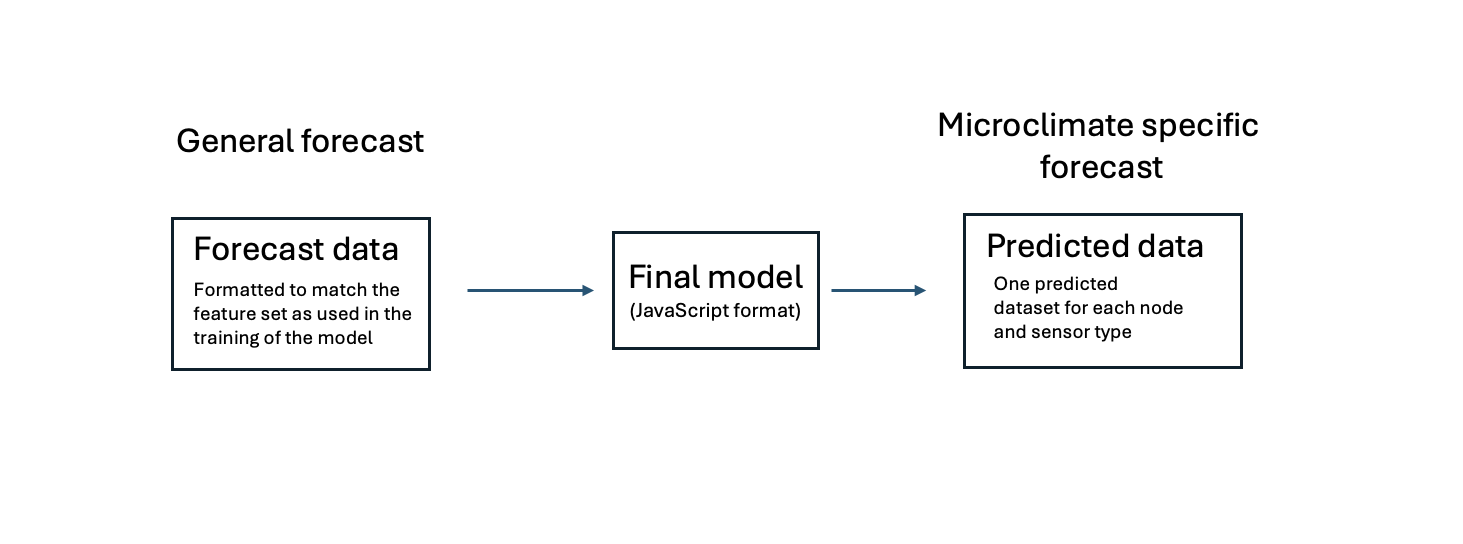
\includegraphics[width=0.8\textwidth]{contents/part-3/fig3/model_diagram.png}
    \caption{Infographic showing how final model is used on the webapp}
    \label{fig:model_diagram}
\end{figure}
